%% Преамбула TeX-файла

% 1. Стиль и язык
\documentclass[utf8x, 12pt]{G7-32} % Стиль (по умолчанию будет 14pt)

% Остальные стандартные настройки убраны в preamble.inc.tex.
\sloppy

% Настройки стиля ГОСТ 7-32
% Для начала определяем, хотим мы или нет, чтобы рисунки и таблицы нумеровались в пределах раздела, или нам нужна сквозная нумерация.
\EqInChapter % формулы будут нумероваться в пределах раздела
\TableInChapter % таблицы будут нумероваться в пределах раздела
\PicInChapter % рисунки будут нумероваться в пределах раздела
\usepackage{slashbox}

% Добавляем гипертекстовое оглавление в PDF
\usepackage[
bookmarks=true, colorlinks=true, unicode=true,
urlcolor=black,linkcolor=black, anchorcolor=black,
citecolor=black, menucolor=black, filecolor=black,
]{hyperref}

% Изменение начертания шрифта --- после чего выглядит таймсоподобно.
% apt-get install scalable-cyrfonts-tex

\IfFileExists{cyrtimes.sty}
    {
        \usepackage{cyrtimespatched}
    }
    {
        % А если Times нету, то будет CM...
    }

\usepackage{graphicx}   % Пакет для включения рисунков

% С такими оно полями оно работает по-умолчанию:
% \RequirePackage[left=20mm,right=10mm,top=20mm,bottom=20mm,headsep=0pt]{geometry}
% Если вас тошнит от поля в 10мм --- увеличивайте до 20-ти, ну и про переплёт не забывайте:
\geometry{right=20mm}
\geometry{left=30mm}


% Пакет Tikz
\usepackage{tikz}
\usetikzlibrary{arrows,positioning,shadows}

% Произвольная нумерация списков.
\usepackage{enumerate}

% ячейки в несколько строчек
\usepackage{multirow}

% itemize внутри tabular
\usepackage{paralist,array}

% Центрирование подписей к плавающим окружениям
\usepackage[justification=centering]{caption}

% Греческий алфавит
\usepackage{upgreek}
% Значки рациональных чисел
\usepackage{amsfonts}


% Настройки листингов.
\ifPDFTeX
% 8 Листинги

\usepackage{listings}
\usepackage{wrapfig}
% Значения по умолчанию
\lstset{
  basicstyle= \footnotesize,
  breakatwhitespace=true,% разрыв строк только на whitespacce
  breaklines=true,       % переносить длинные строки
%   captionpos=b,          % подписи снизу -- вроде не надо
  inputencoding=koi8-r,
  numbers=left,          % нумерация слева
  numberstyle=\footnotesize,
  showspaces=false,      % показывать пробелы подчеркиваниями -- идиотизм 70-х годов
  showstringspaces=false,
  showtabs=false,        % и табы тоже
  stepnumber=1,
  tabsize=4,              % кому нужны табы по 8 символов?
  frame=single
}

% Стиль для псевдокода: строчки обычно короткие, поэтому размер шрифта побольше
\lstdefinestyle{pseudocode}{
  basicstyle=\small,
  keywordstyle=\color{black}\bfseries\underbar,
  language=Pseudocode,
  numberstyle=\footnotesize,
  commentstyle=\footnotesize\it
}

% Стиль для обычного кода: маленький шрифт
\lstdefinestyle{realcode}{
  basicstyle=\scriptsize,
  numberstyle=\footnotesize
}

% Стиль для коротких кусков обычного кода: средний шрифт
\lstdefinestyle{simplecode}{
  basicstyle=\footnotesize,
  numberstyle=\footnotesize
}

% Стиль для BNF
\lstdefinestyle{grammar}{
  basicstyle=\footnotesize,
  numberstyle=\footnotesize,
  stringstyle=\bfseries\ttfamily,
  language=BNF
}

% Определим свой язык для написания псевдокодов на основе Python
\lstdefinelanguage[]{Pseudocode}[]{Python}{
  morekeywords={each,empty,wait,do},% ключевые слова добавлять сюда
  morecomment=[s]{\{}{\}},% комменты {а-ля Pascal} смотрятся нагляднее
  literate=% а сюда добавлять операторы, которые хотите отображать как мат. символы
    {->}{\ensuremath{$\rightarrow$}~}2%
    {<-}{\ensuremath{$\leftarrow$}~}2%
    {:=}{\ensuremath{$\leftarrow$}~}2%
    {<--}{\ensuremath{$\Longleftarrow$}~}2%
}[keywords,comments]

% Свой язык для задания грамматик в BNF
\lstdefinelanguage[]{BNF}[]{}{
  morekeywords={},
  morecomment=[s]{@}{@},
  morestring=[b]",%
  literate=%
    {->}{\ensuremath{$\rightarrow$}~}2%
    {*}{\ensuremath{$^*$}~}2%
    {+}{\ensuremath{$^+$}~}2%
    {|}{\ensuremath{$|$}~}2%
}[keywords,comments,strings]

% Подписи к листингам на русском языке.
\renewcommand\lstlistingname{\cyr\CYRL\cyri\cyrs\cyrt\cyri\cyrn\cyrg}
\renewcommand\lstlistlistingname{\cyr\CYRL\cyri\cyrs\cyrt\cyri\cyrn\cyrg\cyri}

\else
\usepackage{local-minted}
\fi

% Полезные макросы листингов.
% Любимые команды
\newcommand{\Code}[1]{\textbf{#1}}


\begin{document}

\frontmatter % выключает нумерацию ВСЕГО; здесь начинаются ненумерованные главы: реферат, введение, глоссарий, сокращения и прочее.

% Команды \breakingbeforechapters и \nonbreakingbeforechapters
% управляют разрывом страницы перед главами.
% По-умолчанию страница разрывается.

% \nobreakingbeforechapters
% \breakingbeforechapters

% Также можно использовать \Referat, как в оригинале
%\begin{abstract}
%	Титульный лист. Эта страница нужна мне, чтобы не сбивалась нумерация страниц
%	\cite{Dh}
%	\cite{Bayer}
%	\cite{Habr1}
%	\cite{Noise_func}
%	\cite{Ulich}

%Это пример каркаса расчётно-пояснительной записки, желательный к использованию в РПЗ проекта по курсу РСОИ.

%Данный опус, как и более новые версии этого документа, можно взять по адресу (\url{https://github.com/rominf/latex-g7-32}).

%Текст в документе носит совершенно абстрактный характер.
%\end{abstract}
% НАЧАЛО ТИТУЛЬНОГО ЛИСТА
\begin{center}
	\hfill \break
	\textit{
		\normalsize{Государственное образовательное учреждение высшего профессионального образования}}\\ 
	
	\textit{
		\normalsize  {\bf  «Московский государственный технический университет}\\ 
		\normalsize  {\bf имени Н. Э. Баумана»}\\
		\normalsize  {\bf (МГТУ им. Н.Э. Баумана)}\\
	}
	\noindent\rule{\textwidth}{2pt}
	\hfill \break
	\noindent
	\makebox[0pt][l]{ФАКУЛЬТЕТ}%
	\makebox[\textwidth][c]{«Информатика и системы управления»}%
	\\
	\noindent
	\makebox[0pt][l]{КАФЕДРА}%
	\makebox[\textwidth][r]{«Программное обеспечение ЭВМ и информационные технологии»}%
	\\
	\hfill\break
	\hfill \break
	\hfill \break
	\hfill \break
	\normalsize{\bf Р А С Ч Ё Т Н О - П О Я С Н И Т Е Л Ь Н А Я\space\space З А П И С К А}\\
	\normalsize{\bf к курсовой работе на тему:}\\
	\hfill \break
	\large{Метод сохранения качества изображений при понижении его разрядности}\\
	\hfill \break
	\hfill \break
	\hfill \break
	\hfill \break
	\hfill \break	
	\normalsize {
		\noindent
		\makebox[0pt][l]{Студент}%
		\makebox[\textwidth][c]{Капустин А.И.}%
		\makebox[0pt][r]{{$\underset{\text{(Подипсь, дата)}}{\underline{\hspace{8cm}}}$ \space И.О. Фамилия}}
	}\\
	\hfill \break	
	\normalsize {
		\noindent
		\makebox[0pt][l]{Руководитель курсового проекта}%
		\makebox[\textwidth][c]{        Оленев А.А.}%
		\makebox[0pt][r]{{$\underset{\text{(Подпись, дата)}}{\underline{\hspace{6cm}}}$ \space И.О. Фамилия}}
	}
	\hfill \break
	\hfill \break
	\hfill \break
	\hfill \break
\end{center}
\hfill \break
\hfill \break
\begin{center} Москва 2016 \end{center}

\thispagestyle{empty} % 
% КОНЕЦ ТИТУЛЬНОГО ЛИСТА


%%% Local Variables: 
%%% mode: latex
%%% TeX-master: "rpz"
%%% End: 

\tableofcontents


%%% Local Variables:
%%% mode: latex
%%% TeX-master: "rpz"
%%% End:

%\Abbreviations %% Список обозначений и сокращений в тексте

%%% Local Variables:
%%% mode: latex
%%% TeX-master: "rpz"
%%% End:


\Introduction

Задача поиска аномалий относится к одному из популярных способов машинного обучения - обучению без учителя. В настоящее время задачу поиска аномалий активно решают во многих областях жизнедеятельности:
\begin{enumerate} 
	\item Защита информации и безопастность
	\item Социальная сфера и медицина
	\item Банковская и финансовая отрасль
	\item Распознавание и обработка текста, изображений, речи
	\item Другие сферы деятельности(например, мониторинг неисправностей механизмов)
\end{enumerate}
Задачей поиска выбросов, как частный случай задачи поиска аномалий так же занимаются во вышеперичисленных отраслях. 

Количество данных в мире удваивается примерно каждые два года. Поэтому актуальной задачей является разработка новых методов и усовершенствования старых методов поиска выбросов.

В данной работе предлагается новый метод, позволяющий найти аномалии в выборках данных.






\mainmatter % это включает нумерацию глав и секций в документе ниже

\chapter{Аналитический раздел}
\label{cha:analysis}
\section{Цель и задачи работы}
Целью данной работы является создание программного комплекста для обнаружения выбросов временных рядов в собираемых данных.
Для достижения данной цели необходимо решить следующие задачи:
\begin{itemize}
	\item пронализировать предметную область и существующие методы обнаружения выбросов
	\item разработать метод обнаружения выбросов
	\item создать ПО, собирающее данные для анализа
	\item создать ПО, реализующего  разработанный метод обнаружения выбросов
	\item провести вычислительный эксперимент с использованием разработанного метода
	
\end{itemize}
\section{Что такое аномалия}
В анализе данных есть два основных направления, которые занимаются поиском аномалий - это детектирование новизны и обнаружение выбросов. "Объект новизны"\ - это так же объект, который отличается по своим свойствам от объектов  выборки. Однако, в отличие от выброса,  его ещё нет в самой выборке и задача анализа сводится к его обнаружению при появление. Например, если анализировать замеры уровня шума и отбрасывать слишком высокие или слишком низкие значения, то это называется борьбой с выбросами. А если  создаётcя алгоритм, который для каждого нового замера оценивает, насколько он похож на прошлые, и выбрасывает аномальные, то это  назвается "борьбой с новизной"\ .
\cite{Book01}.
Выбросы являются следствием:
\begin{enumerate}
	\item ошибок в данных
	\item неверно классифицированных объектов
	\item присутсвием объектов других выборок
	\item намеренным искажением данных
\end{enumerate}
На рисунке \ref{fig01} находится три вида точек: зеленые, желтые, красные. Множество зеленых точек представляют собой "нормальные" данные. Множество желтых точек означает  выбросы в "слабом смысле". Они незначительно отклоняются от основных  нормальных данных. Красные же точки являются аномальными - выбросами "в сильном смысле"\ . Они значительно  отклоняются  от нормальных данных. В данной работе будет изучаться вопрос находждения "сильных выбросов"\  и  критериев отличия сильного выброса от основных данных. В дальнейшем под словом "выброс"\ будет подразумеваться "сильный выброс"\ ,  а под  аномалией -  выброс(выброс - частный случай аномалии).
Понятие аномалии  интерпетируют по-разному в зависимости от характера данных. Обычно аномалией назыют некоторое отклонение от нормы. В дальнейшем будет дано несколько более формальных опредений аномалий, специфичных для метода их определений.

\section{Обнаружение аномалий}
В машинном обучении обнаружение  "ненормальных" экземпляров в наборах данных всегда представляло большой интерес. Вероятно, первое определение было дано Граббсом\cite{Book02} в 1969 году: "Относительное наблюдение или выброс - это элемент выборки, который, заметно отличается от других членов выборки, в которых он встречается ".
Это определение является актуальным и сегодня, но мотивация для обнаружения аномалий изменилась. Тогда основная причина поиска аномалий заключалась в том, чтобы удалить выбросы из набора данных для обучения, поскольку   используемые алгоритмы, были весьма чувствительны к выбросам в данных. Эта процедура также называется очищением данных. После разработки классификаторов устойчивых к наличию аномалий в обучающем наборе данных, интерес к их поиску угас. Однако, в начале 21 века в связи с развитием интернета и значительным увеличением объема собираемых данных для анализа, исследователи стали больше интересоваться  аномалиями, поскольку они  оказывались часто связаны с особенно интересными событиями.  В этом контексте определение Граббса также было расширено, так что сегодня аномалии имеют две важные характеристики:
\begin{enumerate}
	\item Аномалия отличается от нормы по своим особенностям
	\item Аномалия редко встречается в наборе данных по сравнению с "нормальными"\  данными
\end{enumerate}
\subsection{Классификация методов обнаружений аномалий}
Классическая система классификации предполагает предварительное обучение на обучающем наборе данных и последующую классификацию на основе этого набора. Данные делятся на "обучающую выборку"\ - данные, при помощи которых алогритм обучает классификар и, "тестовую выборку"\ - данные, при анилизе которых, классификатор остается неизменным.Тестовая выборка нужна для того чтобы проверить корректность обучения классификатора.

 Однако, в случае с поиском аномалий, возможны варианты, отличающиеся от классического. Подходящий метод классификации выбирается на основе наличия разметки данных.   Выделяются три основых класса методов:
\begin{enumerate}
\item Обучение с учителем. Для обучения необходимо наличие полностью  размеченных данные для обучения и для тестов. Классификатор  обучается один раз и применяться впоследствии.В связи с тем, что для многих наборов данных заранее неизвестно что является аномалией, а что нет, применение этого метода ограничено.
\item Обучение с частичным привлечением учителя. Для обучения необходимо наличие тествого и учебного набора данных. Однако, в отличие от обучения с привелечением учителя, разметка данных не требуется. Все данные, представленные в выборках, считаются нормальными. На основе этих данных строится некая модель. Все данные, отклоняющиеся от этой модели, считаются аномальными. Эта идея также известна как "одноклассовая" классификация \cite{Book03}.
\item Обучение без учителя.
Самый гибкий способ, который не требует разметки набора данных.  Идея заключается в том, что алгоритм обнаружения аномалий оценивает данные исключительно на основе внутренних свойств набора данных что является нормальным, а что является выбросом. В этой работе основное внимание будет этому  именно этому способу. Так же этот способ называют "неконтролируемый способ обнаружения  аномалий".
\end{enumerate}

\section{Результат метода обнаружения аномалий}
В результате работы алгоритма обнаружения аномалий  с элементом данных связаывается  метка или оценка достоверности(показатель аномальности).  Метка- показатель, который принимает нулевое значения, в случае если она связана с нормальными данными и единицу в противном случае. Оценка показывает вероятность того, что элемент является аномалией. Для разных алгоритмов используется разные шкалы оценок, поэтому приведение конкретных примеров оценок будет некорректным.  В алгоритмах метода обучения с учителем зачастую используются метки как выходные данные, в  алгоритмах  с частичным привлечением учителя и без учителя  обнаружения аномалий чаще встречаются оценки.
\section{Виды аномалий}
\begin{figure}
	\centering
	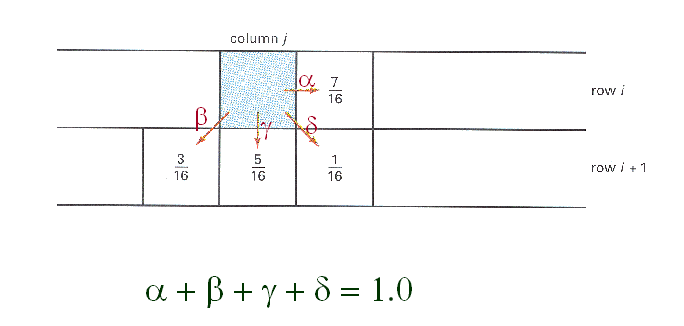
\includegraphics[width=.5\textwidth]{img/1.png}
	\caption{Простой двумерный пример}
	\label{fig01}
\end{figure}

Основная идея алгоритмов обнаружения аномалий заключается в обнаружении экземпляров данных в наборе данных, которые отклоняются от нормы. Однако на практике существует множество случаев, когда это основное предположение является неоднозначным. На рис \ref{fig01} показаны некоторые из этих случаев с использованием простого двумерного набора данных. Две аномалии могут быть легко идентифицированы визуально: красные точки  сильно отличаются отличаются значениям параметров от областей плотной группировки точек. Если смотреть на весь набор данных в целом, то фиолетовую точку можно отнести к тому же классу, что и зеленые точки.  Однако, если сфокусироваься только на кластере зеленых точек и сравнивать его с фиолетовой точкой, пренебрегая всеми другими точками, то её можно рассматривать как аномалию. Поэтому фиолетовая точка называется локальной аномалией, так как она аномальна по сравнению с ее близкой окрестностью. В зависимости от цели анализа, локальные  аномалии могут представлять интерес или нет. 
Другой  вопрос  заключается в том,что следует ли рассматривать точки черного кластера  как три аномалии или как (небольшой) кластер. Такие небольшие кластеры явления называются микрокластерами. Показатели аномальности у точек этого кластера выше, чем  у точек зеленого кластера, но меньше, чем  у красных точек. Этот простой пример  показывает, что задача нахождения аномалий аномалии не всегда тривиальна, а вычисление показателя аномалности иногда полезнее, чем проставление двоичной метки.


Задача обнаружения одиночных аномальных экземпляров  крупном наборе данных называется обнаружением точечных аномалии\cite{Book04}. Сегодня почти все  неконтролируемые алгоритмы обнаружения  относятся к этому типу. Если же аномалии составляют заметный процент, от набора данных, то задачу поиска аномалий называют задачей обнаружения коллектнивных аномалий. Пусть аномалии представляют собой некое множество, тогда необязательно каждый элемент этого множества должен быть аномальным. Возможен вариант когда только определенная их комбинация определяет аномалию.  Третий вид  -  контекстуальные аномалии. Элемент выборке в отрыве от своего контекста может казаться нормальным. Однако, если рассмотреть контекст этого элемента, то очевидным станет его аномальная природа.
 Распространенным контекстом является время. В качестве примера предположим, что  измеряется температура в диапазоне от $-30^{\circ}$C до $+40^{\circ}$C в течение года. Таким образом, температура $25^{\circ}$C кажется довольно нормальной, но когда  учитывается контекстное время (например, месяц), такая высокая температура $25^{\circ}$C  в течение зимы  будет рассматриваться как аномалия.

Алгоритмы обнаружения точечных аномалий так же можно использовать для обнаружения контекстуальных и коллективных аномалий. Для этого нужно включить контекст в алгоритм как параметр алгоритма. В вышеприведенным примере включение месяца как дополнительного параметра поможет обнаружить аномалию. Однако в более сложных сценариях может потребоваться один или несколько новых парметров, чтобы преобразовать задачу определения контекстной аномалии в задачу обнаружения точечной аномалии.  Для того, чтобы преобразовать задачу поиска коллективной аномалии в задачу поиска одиночной, нужно произвести измненения изначального набора данных. Для этого можно использовать корреляцию, агрегация и группировка. Преобразование  может быть нетривиальным.\cite{Book05} . 
Преобразование требует глубоких знаний о наборе исходных данных и часто приводит  к существенным искажениям при переводе данных в новый формат. Такое семантическое преобразование называется  генерированием представления данных(\textit{англ. data view generation}).
  
  Таким образом можно сделать вывод, что многие задачи обнаружения аномалий требуют предварительной обработки данных перед передачей их на вход алгоритму. В противном случае можно получить формально верные, но фактические бесполезные результаты.
\subsection{Нормализация данных} 
После получения предварительно обработанного датасета для поиска точечной аномалии, то последним шагом перед передачей в алгоритм, является нормализация данных. Нормализация данных предназначена для устранения зависимости от выбора единицы измерения и заключается в преобразовании диапазонов значений всех атрибутов к стандартным интервалам([0,1] или [-1,1])\cite{Book06}. Нормализация данных направлена на придание всем атрибутам одинакового "веса".
\subsubsection{Основные методы нормализация данных}
\begin{enumerate}
	\item Min-max нормализация заключается в применении к диапазону значений атрибута х линейного преобразования, которое отображает [min(х),max(х)] в [A,B].
	\begin{equation}
	x^\prime_i=\uptau(x_i)=\frac{x_i - min(x)}{max(x) - min(x)}*(B-A) + A
		\end{equation}
   \begin{equation}
		x \in[min(x), max(x)] \Rightarrow \uptau(х) \Rightarrow [A,B]
	\end{equation}
	Min-max нормализация сохраняет все зависимости и порядок оригинальных значений атрибута. Недостатком этгого метода является то, что выбросы могут сжать основную массу значений к очень маленькому интервалу
	\item Z-нормализация  основывается на приведении распределения исходного атрибута х  к центрированному распределению со стандартным отклоненим, равным 1 \cite{Book06} .
	\begin{equation}
	x^\prime_i=\uptau(x_i) =\frac{x_i - \overline{x}}{\sigma_x}
		\end{equation}
		\begin{equation}
		M[x^\prime]=1	 
		\end{equation}
		\begin{equation}
		D[\overline{x}^\prime]=0	 
		\end{equation}
		Метод полезен когда в данных содержатся выбросы.
	\item Масштабирование заключается в изменении длины вектора значений атрибута путем умножения на константу \cite{Book06} .
	\begin{equation}
	x^\prime_i=\uptau(x_i)=\lambda*x_i
	\end{equation}
	Длина вектора х уменьшается при $|\lambda|<1$ и увеличивается при $|\lambda|>1$ 
\end{enumerate}
\section{Неконтролируемые алгоритмы обнаружения аномалий}
\subsection{Вероятностный-генеративный подход}
Основная идея генеративного подхода заключается в использование вероятностного смесевого моделирования данных. Предлагается подобрать такую вероятностую модель, из которой было получены нормированные данные. Такие модели обычно называются генеративными моделями, где для каждой точки(элемента данных) можем посчитать генеративную вероятность(или вероятность правдоподобия).Т.е. задача  сводится к нахождению плотности распределения p(x). Аномалиями при этом  считаются точки(элементы набора данных), имеющию низкое правдоподобие. В качестве показателя аномальности выступает функция p.
Для построения генеративной модели нужно решить следующую задачу:
	\begin{equation}
	\prod \limits_{x \in X_{norm}} p(x,\theta)  \rightarrow max_\theta
		\end{equation}
		где $ X_{norm}$ - нормальные данные представленного набора данных ${p(x,\theta)|\theta \in \omega}$ -семейство плотностей вероятностей, параметризованные $\theta$;
		
Этот метод редко используется на практике, так как тяжело проверить полученную генеративную модель на адекватность, сложно  убедится в правильном выборе семейства смесевых распределений. Это связано с тем, что низкое значение функции правдоподобия может означать как и аномальное значение, так и неудачно подобранную модель. Этот метод применяется с опорой на априорную информацию, в случае когда можно проверить полученную модель на адекватность.
\subsection{Линейный подход}
Основной идей линейного подхода является построение некой  модели, характеризующей нормальные данные. Точки, которые значительно отклоняются от этой модели, считаются аномалиями.

Предполагается, что нормальные данные  находятся в подпрострастрансве пространства атрибутов данных(размер подпространства атрибутов данных равен размерности данных). В свою очередь, задача линейного метода - найти низкоразмерное подпространства, такие что, выборка данных этого подпространства значительно отличается от остальных точек пространства данных.

Одним из возможных вариантов решения является использование линейной регрессии. Выбирается одна из наблюдаемых переменных  набора данных и относительно неё решается задача линейной регрессии оставшихся атрибутов. Итоговым ответом будет является усредненное значения показателя аномалии по всем атрибутам. 

Алгоритмы, основанные на линейном подходе, требуют  наличия линейной зависимости атрибутов данных. 
\subsection{Метрические методы}
Мерические методы пытаются найти в данных точки, в некотором смысле
изолированные от остальных\cite{Book01}. Если в пространстве задана некоторая метрика \textit{p(x1, x2)}, то необходимо задать следующие понятия:
\begin{itemize}
	\item  Аномалии – точки, не попадающие ни в один кластер. К данным применяется один из алгоритмов кластеризации; размер кластера, в котором оказалась точка, объявляется её показатель аномальности.
	\item Локальная плотность в аномальных точках низкая. Для данной точки показателем аномальности объявляется локальная плотность, которая оценивается некоторым непараметрическим способом.
	\item Расстояние от данной точки до ближайших соседей велико.
\end{itemize}
 В качестве показателя аномальности может выступать:
 \begin{itemize}
\item расстояние до k-го ближайшего соседа;
\item среднее расстояние до k ближайших соседей;
\item медиана расстояний до k ближайших соседей;
\item гармоническое среднее до k ближайших соседей;
\item доля из k ближайших соседей, для которых данная точка является не
более чем k-ым соседом и много другое.
\end{itemize}
\subsubsection{Базовые понятия}
Метрические методы хорошо подоходят в случае когда данные не размечены. Сложность вычисления прямо пропорциональна как размерности данных m,как и их количеству n. При росте набора данных наблюдается экспоненциальный рост сложности вычислений. Однако, эти методы хорошо проявляют себя на ограниченных наборах данных\cite{Book07}. Следовательно такие методы как k-ближайших соседей(так же известный как обучение на основе примеров, и описанный поздее) с нотацией ассимтпотического роста $O(n^2m)$ недопустимы для наборов данных с большой размерности, если их размерность не может быть уменьшена.

Существуют много  различных вариации алгоритма k-ближайших соседей для обнаружения аномалий, но все они основаны на вычислении некой метрики "расстояния до соседей", такой как Евклидово расстояние или  расстояние Махаланобиса. Евклидово расстояние задается следующей формулой:
 	\begin{equation}
 	\sqrt{\sum_{i=1}^n(x_i-y_i)^2}
 		\end{equation}
 и является просто расстоянием между двумя точками, когда как  расстояние Махаланобиса, задаваемое следующей формулой
 	\begin{equation}
 	\sqrt{(x-\mu)^T C^-1 (x-\mu)}
 	\end{equation}
 	вычисляет расстояние от точки до центра тяжести ($\mu$), определяемого формулой коррелированных атрибутов, заданных матрицей ковариации (C). Расстояние  Махаланобиса
 	рассчитывается значительно дольше по сравнению с евлидковым
 	 по сравнению с евклидовым расстоянием для для больших объемов данных, поскольку оно требует
 	пройти через весь набор данных, чтобы идентифицировать корреляции атрибутов.

 \subsubsection{Оптимизация Рамасвани} 	
 Точка p является выбросом,
если не более n - 1 других точек в наборе данных имеют более высокий $D_m$(расстояние до m соседей), где m задается. Например на рисунке \ref{fig02} черная точка является наиболее удаленной от соседей, следовательно она является выбросом. Красные точки расположены рядом друг с другом, однако расстояние до других точек велико, следовательно они тоже являются аномалиями. Такой подход воприимчив к вычислительному росту, потому что должна быть вычислена матрица расстояний точек друг от друга, поэтому Рамасвани в 2000 году предложил оптимизацию метода k-ближайших соседей(c англ. k-Nearest Neighbour - k-NN)  в виде составления ранжированного списка потенциальных выбросов.
\begin{figure}
	\centering
	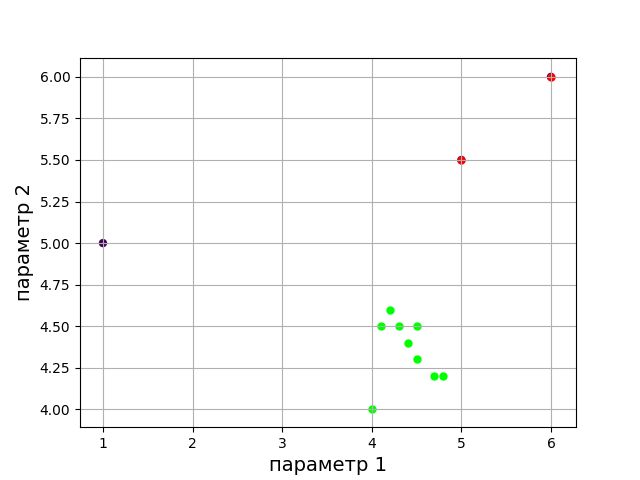
\includegraphics[width=.5\textwidth]{img/2.png}
	\caption{Пример k-ближайших соседей}
	\label{fig02}
\end{figure}

 Оптимизация Рамасвани заключается в разбиении данных на ячейки.Если какая-либо ячейка и ее ближайшие соседи содержат больше, чем k
 точек, то точки в ячейке считаются лежащими в плотной области
 поэтому содержащиеся там точки вряд ли будут выбросами. Если же почти все ячейки содержат больше,чем k точек, а какие-то ячейки содержат меньше, чем k точек, то тогда все точки, лежащие в ячейках, которые содержат  менее k элементов, помечаются  аномальным. Следовательно,
 необходимо обработать только небольшое количество ячеек, которые ранее не были помечены и только относительно небольшое количество расстояний необходимовычислить для обнаружений аномалий. 
 \subsection{K ближайших соседей}
 Алгоритм работы метода:
 \begin{itemize}
 	\item Выбирается число K-число соседей, относительно
 	\item Устанавилается граница показателя аномальности, на основе которой будет определятся метка элемента(задается в процентах относительно среднего показателя расстояния)
 	\item На основе метрики, рассчитывающей расстояния между элементами, высчитается расстояние между всеми элементами и всеми его соседями.
 	\item Полученный результат сортируется на 
 	\item На основе полученных расстояний и границы показателя аномальности элементам присваиваются метки.
 \end{itemize}
 В качестве метки, рассчитывающей расстояния между элементами можно использовать следующую формула:
 \begin{equation}
 L=\sum_{0}^{k}x_j0 - x_ji
 \end{equation}
 где $x_ji$ - значение j-того атрибута элемента до которого ищется расстояние, а $x_0$-искомый элемент.
 
 \subsubsection{Методы Кнора-Реймонда и Байерса-Рейтери}
 Кнор и Реймонд предложили свой эффективный метод  КНН подхода обучения без учителя\cite{Book09}. Если m из k ближайших соседей (где m<k) лежат
 в пределах определенного порогового значения d, тогда  считается, что  данные точки лежат в достаточно плотной области распределения данных, подлежащей классификации и подлежат классификации как нормальные, в противном случае они помечаются как аномальные.
 
  Очень похожий метод был придуман для идентефикации  наземных мин  на спутниковых снимках поверхности Земли Байеросом с соавторстве с Рейтери\cite{Book10}(этот метод можно использовать и для других целей) Он заключается в том, что берется m точек, для них ищется расстояние $D_m$. Если расстояние меньшего некого порогового значеня d,тогда  считается, что  данные точки лежат в достаточно плотной области распределения данных, подлежащей классификации и подлежат классификации как нормальные, в противном случае они помечаются как аномальные. Этот метод уменьшается количество варьируемых параметров, по сравнению с методом Кнора-Реймонда: остаются только параметры d и m, параметр k убирается. 
  подход оригинальный подход k-NN, поскольку только k ближайших соседей должны быть вычислены для каждой точки, а не всей матрицы расстояния
  для всех точек
\subsection{Метод Танга}
Метод Танга заключается  в вычислении средней цепочку расстояний между точкой p и k её соседями. Ранним расстояниям присваиваются более высокие веса, поэтому, если точка находится в разреженной
области как черная точка на рисунке\ref{fig02}, то путь до  ее ближайших соседей  будет относительно далеким, а среднее расстояние цепочки
будет высоким. Этот метод выгодно отлчичается от вышеописанных тем, что учитывает как  плотность, так и изоляцию. Рассмотрим рисокок \ref{fig03}.
Очевидно, что черные точки являются аномалиями, а скопление зеленых точек - множеством "нормальных" точек. Однако, алгоритмы k-NN классификации могут столкнутся с проблемой того, что расстояние от черных точек до зеленого кластера примерно равно, значит эти точки можно отнести к одной группе и при определенных значениях параметров алгоритма эти точки не будут считаться аномалиями. Метод Танга поможет избежать таких ошибок при обнаружении выбросов.
\begin{figure}
	\centering
	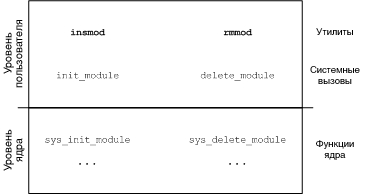
\includegraphics[width=.5\textwidth]{img/3.png}
	\caption{Пример для метода Танга}
	\label{fig03}
\end{figure}
 Однако метод является вычислительно сложным с временем выполнения как у оринального k-NN, поскольку он полагается на вычисление путей между всеми точками и их k соседей. 
\subsection{Параметрическе методы}
Вышеописанные методы плохо подходят для работы с большим объемом данных.
Параметрические методы позволяют очень быстро пересчитывать модель для
новых данных и подходит для больших наборов данных; модель растет
только с сложностью модели, а не размером данных. Однако они ограничивают
применимость,  применяя предварительно выбранную модель распределения для проверки данных на аномальность. Т.е. предварительно априорно подбирается модель правдоподобности данных. Элементы , которые значительно отклоняются от этой модели считаются аномальными. Параметрический подход схож с линейным по описанию, но значительно отличается от него по принципу работы.

Одним из таких подходов является оценка эллипсоидой минимального объема\cite{Book11}, которая соответствует наименьшему допустимому эллипсоиду, покрывающему не меньше 50\% точек выборки.
\begin{figure}
	\centering
	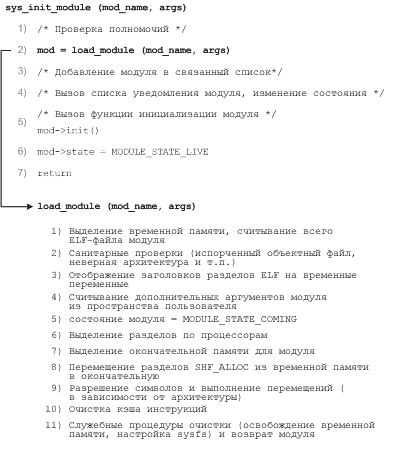
\includegraphics[width=.5\textwidth]{img/4.png}
	\caption{Двухмерная проекция эллипсоиды минимального объема}
	\label{fig04}
\end{figure}
\subsection{Локальный коэффициент выбросов(LOF)}
Этот метод является одним из самых известных алгоритмов обнаружения локальных аномалий. Недостатком метрических методов является тот факт, что все лежащие в их основе предположения верны лишь в дополнении друг с другом: локальная плотность точки, лежащей в центре небольшого кластера аномалий, может оказаться выше, чем для любой точки из большого кластера
нормальных данных. Возможно и обратное: изолированная точка-аномалия может располагаться, например, в центре масс кластера нормальных точек, и тогда среднее расстояние от неё до соседей будет меньше, чем для нормальных точек. Это "свойство" метрических алгоритмов пытается учесть алгоритм  локального коэффициентов выбросов(англ.Local Outlier Factor).

Чтобы вычислить LOF необходимо произвести следующие действия:
\begin{enumerate}
\item Для каждой записи найти всех соседей, расстояния до которых не превышает k. Их количество может быть больше, чем k.
\item Использую эти записи для каждой точки $N_k$, вычислить локальную плотность точки, основанную на локальной плотности достижимости(англ. local reachability density (LRD)):
\begin{equation}
LRD_k(x) = 1/(\frac{\sum_{o \in N_k(x)}d_k (x,o)}{|N_k (x)|})
\end{equation}
где $d_(x,o)$ расстояние достигаемости. За редким исключеним в качестве расстояния достигаемости используется евклидово расстояние \cite{Book12}
\item Вычисляем LOF путем сравнения LRD записи с LRD соседей.
\begin{equation}
LOF(x) = \frac{\sum_{o \in N_k(x)}\frac{LRD_k (o)}{LRD_k (x)}}{|N_k (x)|}
\end{equation}
\end{enumerate}
Таким образом LOF является отношением локальных плотностей.  Нормальные записи, плотности которых равны плотности их соседей, получают оценку около 1,0. Аномалии, которые имеют низкую локальную плотность, получат значительно более высокую оценку. Алгоритм полагаясь только на свою прямую окрестность,формирует  оценку - величину, основанную основанное только на k-соседях. Конечно, глобальные аномалии также могут быть обнаружены, так как они  имеют низкую LRD,по сравнению со своими соседями. Важно отметить, что в задачах обнаружения аномалий, где местные аномалии не представляют интереса, этот алгоритм будет генерировать множество ложных аномалий Hастройка k имеет решающее значение для этого алгоритма.

Авторы алгоритма LOF рекомендуют использовать для вычисления k стратегию ансамблирования( алгоритм описан ниже). Берется интервал возможных значений k и с некоторым шагом для всех возможных значений k вычисляется показатели аномальности для каждого элемента выборки. Путем голосования определяется является ли эта ли эта точка аномалий. Однако, на практике такие рекомендации редко исользуют из-за их значительной вычислительной сложности.
\subsubsection{Компонентный коэффициент выбросов(COF)}
\begin{figure}[h!]
	\centering
	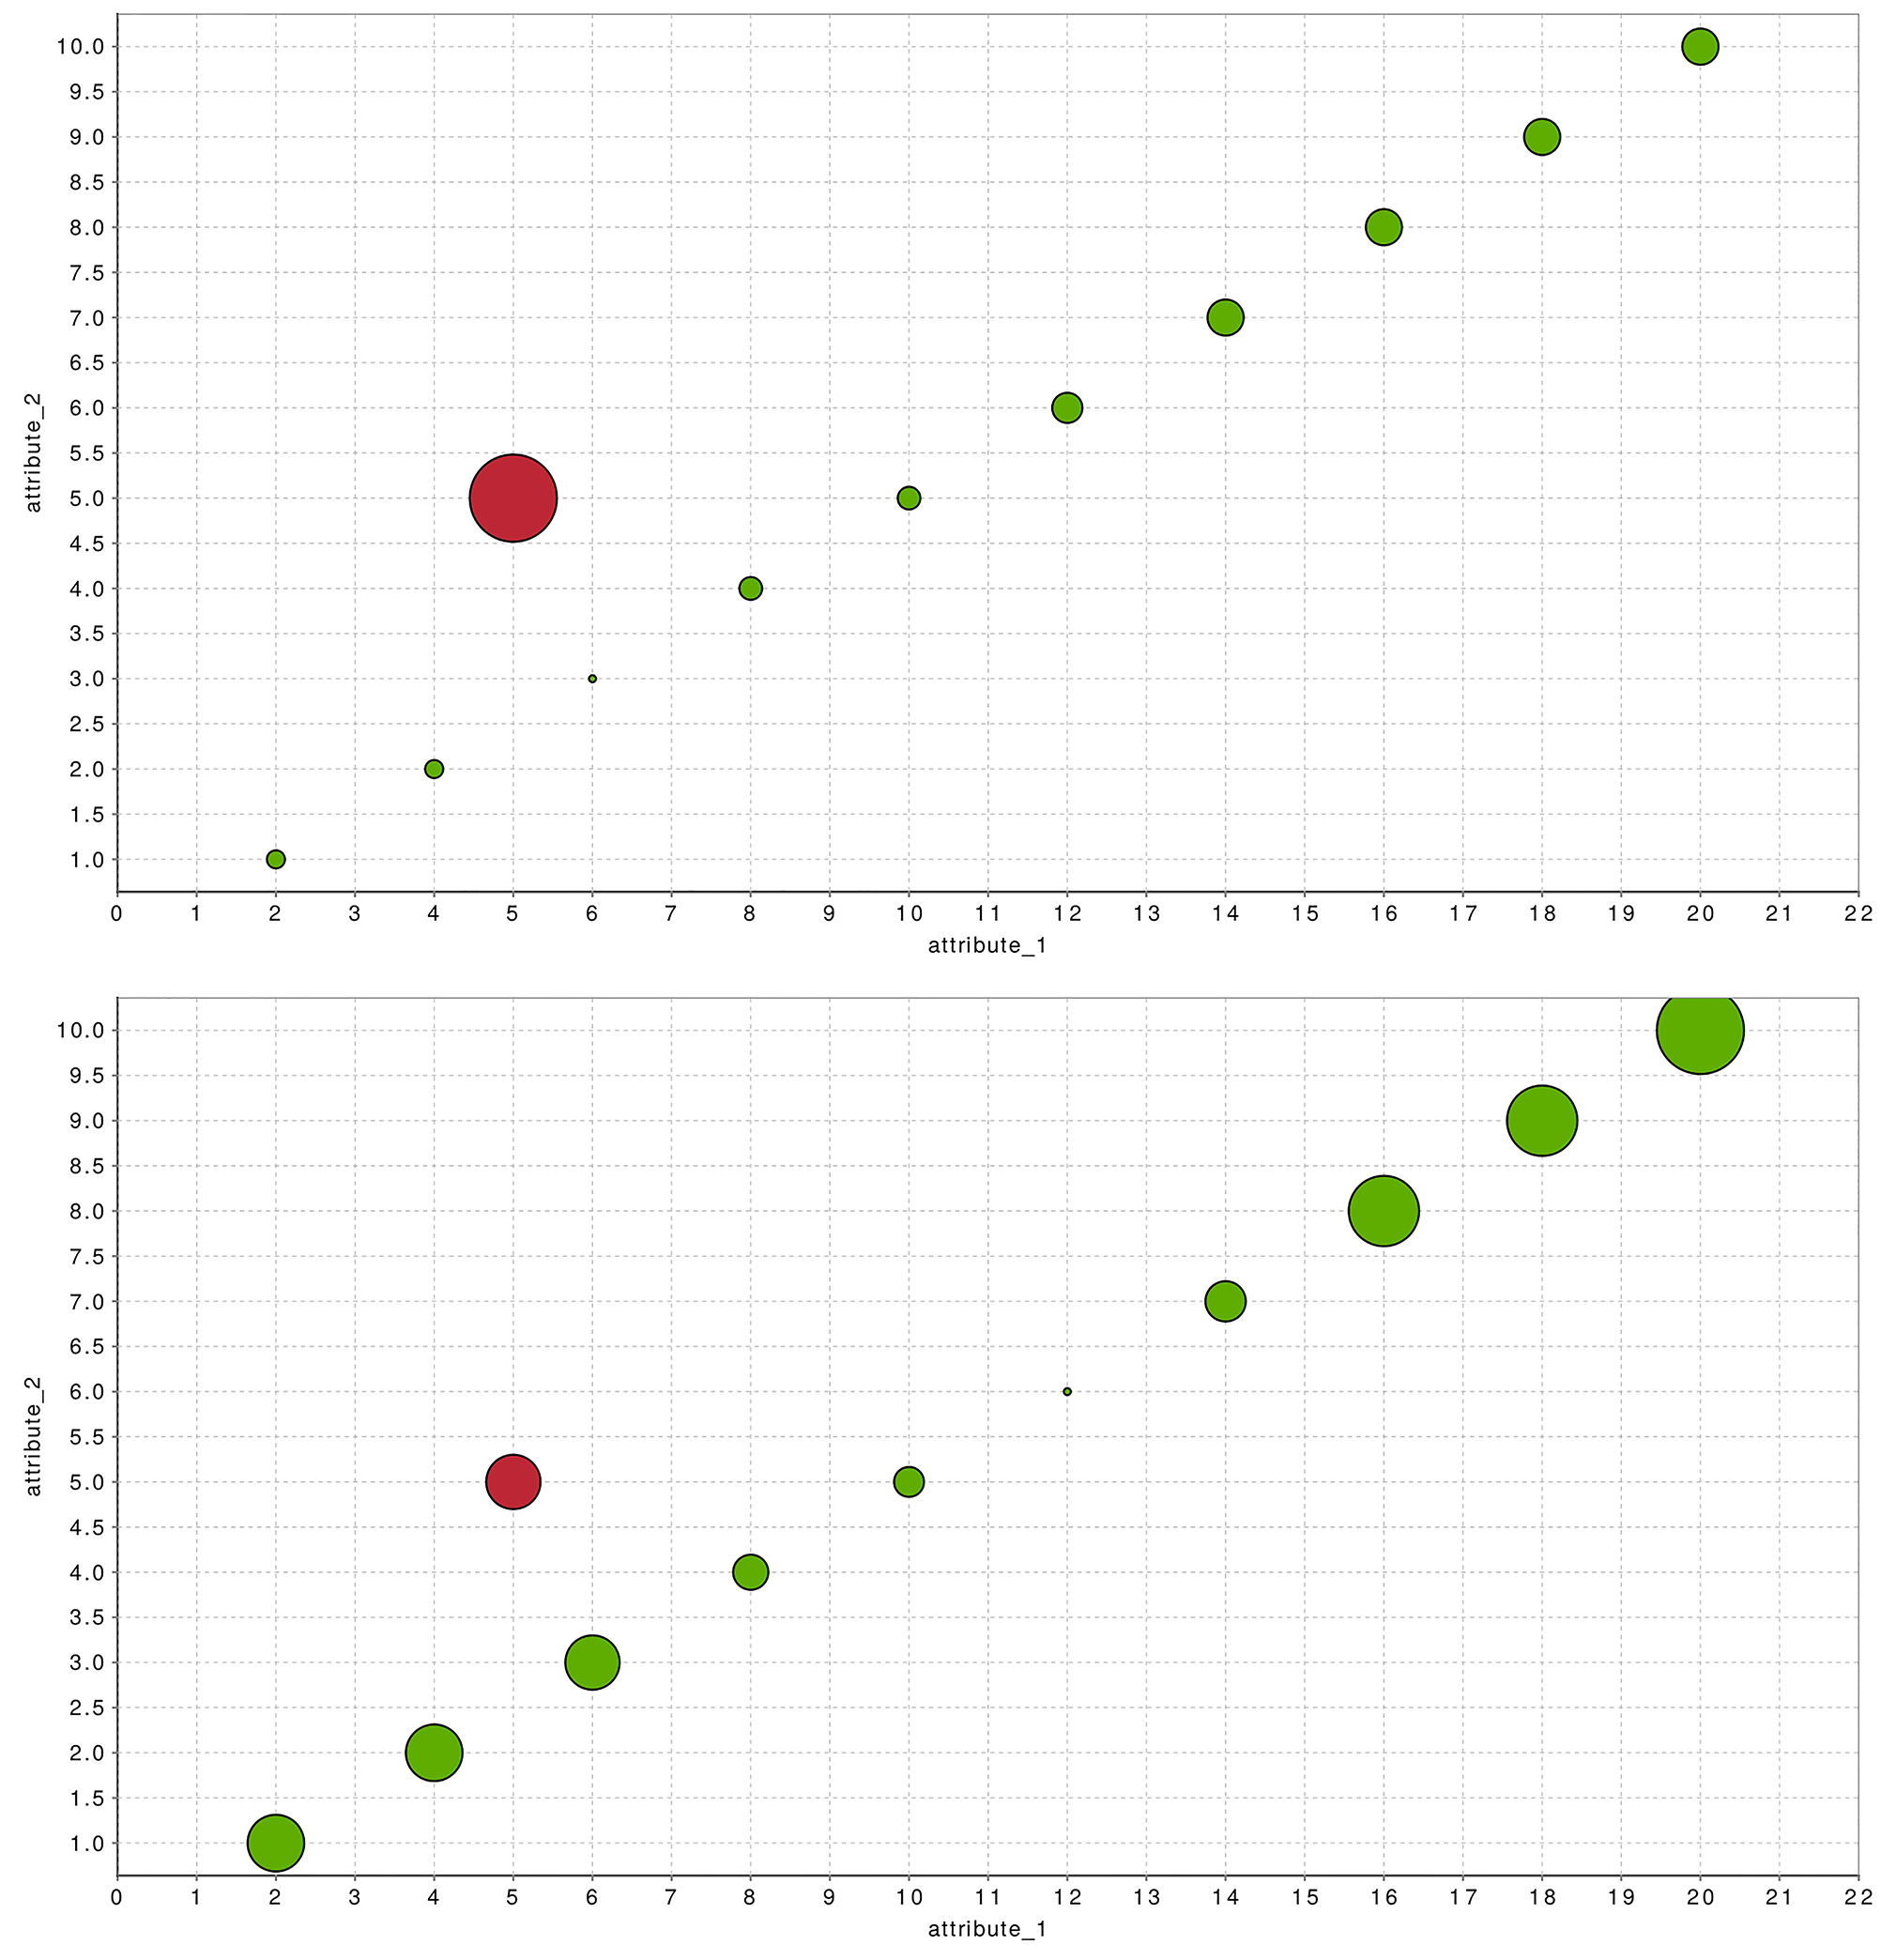
\includegraphics[width=.5\textwidth]{img/5_3rdpart.png}
	\caption{Сравнение COF (сверху) с LOF (внизу) с использованием простого набора данных с линейной корреляцией двух атрибутов}
	\label{fig05}
\end{figure}
Компонентный коэффициент выбросов аналогичен LOF, но оценка плотности для записей выполняется иным способм В LOF k-ближайших соседей выбирают на основе евклидова расстояния. Это косвенно предполагает, что данные распределяются сферическим образом вокруг экземпляра. Если это допущение нарушено, например, если функции имеют прямую линейную корреляцию,то оценка плотности неверна. COF исправляет этот недостаток и оценивает локальную плотность окрестности с использованием метода кратчайшего пути, называемого расстоянием цепочки. Математически это расстояние цепочки является минимумом суммы всех расстояний, соединяющих все k соседей точки и саму точку. Например, когда функции, очевидно, коррелированы, этот подход оценки плотности работает значительно лучше \cite{Book14}. 
На рисунке 5 показан результат для LOF и COF в сравнении для простого двумерного набора данных, где атрибуты имеют линейную зависимость. Можно видеть, что оценка  плотности LOF не может обнаружить выброс, но COF удадается связать  нормальные между собой для оценки локальной плотности.


\section{Методы улучшения алгоритмов}
\subsection{Cемпилрования}
Большинство алгоритмов распознавания аномалий успешно работают на вы-
борках малых размеров. Поэтому предлагается разбить начальный набор данных на несколько случайных выборок и усреднить результат. Размер этих выборок может быть как и случайным, там и фиксированного размера, но, как правило, он отличается от размеров исходного набора данных не меньше чем на порядок. Идея такого выбора заключается в том, что шумовые объекты попадут в выборки с низкой вероятностью; кластера нормальных данных будут представлены несколькими представителями, а кластера аномалий выродятся в изолированные точки. На основе этих выборок алгоритмы строят функции показателя аномальности, незначительно уступующему результату, полученному на основе анализа всех исходных данных. 

Этот метод помогает значительно сократить вычислительную сложность, а так же уменьшить вероятность "подгона" алгоритма под конкретный набор данных.  В силу особенностей задачи, необходимое условие отсут-
ствия параметризации алгоритмов зачастую означает их детерминированность(в отсутсвиее стохастичности показатель аномальности однозначно определяется по  заданной выборке). В общем случае при добавлении новых данных в общий набор данных, можно не пересчитывать заново показатель аномальности для всего набора данных, а добавить запуски алгоритма на новых данных в ансамбль(так называемый warm start\cite{Book15})
\subsection{Ансамблирование голосованием}
Ансамблированием в задаче поиска аномалий называют использование нескольких различных алгоритмов с последующи усреднением их показателя аномальности. При использовании различных классов алгоритмов можно столкнуться с проблемой того, что показатель аномальности выглядит по-разному в различных алгоритмах и сравнить напрямую эти показатели некорректно.  Поэтому традиционное приведение  показателей значений различных функций к одному диапазону, например,к [0,1], будет некорректным.
Существует несколько наиболее известных видов ансамблирования:
\begin{itemize}
	\item Простое голосование 
	\begin{equation}
	b(x)=F(b_1(x),...,b_T(x))=\frac{1}{T}\sum_{t=1}^{T}b_t(x)
	\end{equation}
	\item Взвешенное голосование 
	\begin{gather}
	b(x)=F(b_1(x),...,b_T(x))=\frac{1}{T}\sum_{t=1}^{T}w_tb_t(x)\\
		\sum_{t=1}^{T}w_t=1, w_t \geq 0
	\end{gather}
		\item Cмесь экспертов
		\begin{gather}
		b(x)=F(b_1(x),...,b_T(x))=\frac{1}{T}\sum_{t=1}^{T}w_t(x)b_t(x)\\
		\sum_{t=1}^{T}w_t=1, \forall x\in X
		\end{gather}
 \end{itemize}
	Простое голосование - это  частный случай взвешенного голосования, а взвешенное голосование является частным случаем смеси экспертов. 
	
	Различные методы ансамблирования такие как беггинг, бустинг, стекинг и другие применяются для улучшения работы алгоритмов обучения с учителем \cite{Book16}. Для алгоритмов обучения без учителя применяется простое голосование, т.к. задача изменения весов голосования нетривиальна в задаче обучения без учителя.
\subsection{Итеративный отбор}
Итеративный отбор основам на идее многократного применения алгоритмов ансамблирования. Преположим, построеная некоторая модель, описывающая нормальные данные. Эта модель построена на основе всех  имеющихся данных, но точность этой модели невелика, она умеет определить только явные аномалии. Отсортировав все точки по показателю аномальности, мож-
но выбрать k самых аномальных объекта в данных и исключить из данных. После этого можно перестроить модель и повторить вышеуказанные действия несколько раз, пока не будут достигнуты некоторые условия. При каждой итерации точность модели будет увеличиваться.

Идея итеративного отбора может быть обобщена различными способами. Результат работы одного алгоритма может быть использован для отсеивания явных аномалий и настройки нового алгоритма, не обязательно совпадающего с предыдущим, на оставшихся данных. х. Возможна и противоположная механика: по результатам работы одного алгоритма отбираются явные, гарантированные
представители нормальных данных, и исключительно на них строится модель,
их описывающая
\section{Выводы}
Существует большое число алгоритмов для нахождения аномалий. Некоторые из них опирается на априорные данные, некоторые не опираются. Для выбора подходящего алгоритма нахождения аномалий зачастую стоит учитывать характер данных, их размер и доступную априорую информацию. Несмотря на то, область знаний обнаружения аномалий активно развивается как часть современной науки, остается ещё много простора для исследования алгоритмов, модификации и создания новых.
% Обратите внимание, что включается не ../dia/..., а inc/dia/...
% В Makefile есть соответствующее правило для inc/dia/*.pdf, которое
% берет исходные файлы из ../dia в этом случае.

%\begin{figure}
%  \centering
%  \includegraphics[width=\textwidth]{inc/dia/rpz-idef0}
%  \caption{Рисунок}
%  \label{fig:fig01}
%\end{figure}

%\begin{figure}
%  \centering
%  \includegraphics[height=0.85\textheight]{inc/img/leonardo}
%  \caption{Предполагаемый автопортрет Леонардо да Винчи}
 % \label{fig:leonardo}
%\end{figure}

%В \cite{Pup09} указано, что...


\chapter{Конструкторский раздел}
\label{cha:design}
\chapter{Технологический раздел}
\section{Выбор средств разработки}
\subsection{Выбор целевой платформы}
Программный продукт  не затачивается под работу на конкретной ОС. В качестве целевых платформ разработки были выбраны ОС Windows и Linux, Данный выбор обусловлен широкой распространенностью ОС Windows и Linux, большим количеством средств разработки для данных платформ, что дает возможность выбирать
язык программирования и сопутствующие инструменты, ориентируясь на возможность простого и надежного решения рассматриваемой
задачи, а не на ограничения целевой платформы.


\subsection{Выбор языка программирования}
Для написания комплекса программ создания прогнозов был выбран язык Python.
Python - универсальный мультипарадигменный скриптовый язык программирования. Так же для Python написано большое количество библиотек машинного обучения, а так же для работы с тектовыми данными, что особенно важно для данной работы.
Преимущества данного языка:
\begin{itemize}
	\item Кроссплатформенность. Python – это интерпретируемый язык, его интерпретаторы существуют для многих платформ. Поэтому с запуском его на любой ОС не должно возникнуть проблем.
	\item С Python доступно большое количество сервисов, сред разработки, и фреймворков. Легко можно найти подходящий продукт для работы.
	\item Возможность подключить библиотеки, написанные на С. Это позволяет повысить эффективность, улучшить быстродействие.
\end{itemize}



Так же для работы с данными использовался языка bash. Bash - это мощный и простой в использовании язык сценариев. Он позволяет 	 легко перемещать курсор и редактировать текст команды в командной строке, поддерживает историю команд: дает возможность повторить или при необходимости изменить команду, которая была введена в командной строке ранее. Позволяет легко указать команде, откуда брать входные данные и куда направлять выходные данные. Поддерживаются псевдонимы - создание кратких обозначения для однострочных команд.

\subsection{Выбор среды разработки и отладки}
Из-за использования сразу нескольких языков, в процессе работы над программным комплексом, было использовано несколько сред разработки.
Pycharm - современная кросс-платформенная среда разрабтки, которая предоставляет широкие возможности разработки программ на python, а так же их отладки. Pycharm так же поддерживает работу со сторонними плагинами, что позволило использовать плагин работы с системой контроля версий.

В процессе работы с различными библиотеками приходится сталкиваться с различными языками программирования, например, с С. Для работы с различными вспомогательными языками был использован текстовый редактор Visual Studio Code. Он имеет плагины для поддержки большинства современных языков программирования, а набор плагинов к текстовому редактору позволяет осуществлять запуск и отладку кода прямо из редактора, а так же позволяет осуществлять автоматическое форматирование кода.

Для работы с bash использовался nano - консольный текстовый редактор для Unix и Unix-подобных операционных систем, основанный на библиотеке curses. В настоящее время включен в дистрибутивы Ubuntu по умолчанию и в установке не нуждается.

\section{Система контроля версий}
В процессе разработки программы использовалась система контроля
версий Git.
Система контроля версий позволяет вносить в проект атомарные
изменения, направленные на решения каких-либо задач. В случае
обнаружения ошибок или изменения требований, внесенные изменения
можно отменить.
Кроме того, с помощью системы контроля версий решается вопрос
резервного копирования.
Особенности Git:
\begin{itemize}
\item Предоставляет широкие возможности для управления изменениями
	проекта и просмотра истории изменений
 \item Данная система контроля версий является децентрализованной, что
позволяет иметь несколько независимых резервных копий проекта.
\item Поддерживается хостингом репозиториев GitHub и Gitlab.
\item Поддерживается средой разработки Pycharm и Visual Studio Code.
\end{itemize}

\section{Формат файлов}
На вход программе для осуществления прогнозов подаётся англоязычный текст длинною от 10 до 2000 символов.
\begin{lstlisting}[,,escapeinside={(@}{@)},caption={Пример входных данных для программы оценки тональности текста}, xleftmargin=.1\textwidth, xrightmargin=.1\textwidth] 
I thought I started a little slow, but I thought he played really well today. I knew his game plan, I got onto it pretty quickly. He directed most of his serves to my forehand. He hasn't really done that in the past. It's definitely my weaker return. He was definitely trying to stay away from my backhand return a lot.

But I thought just on big points, I mean, he played well. Hit his forehand extremely well. When Rafa plays well, he hits his forehand line extremely well. I thought today he was on fire with that shot. Every time he redirected, he was hitting balls just within the line, so...

I thought it was a high-level match. Two tiebreaks. I played a couple loose points here or there. That's all it takes against a player like that. He was just too good today.
\end{lstlisting}

Так же программе на вход подаются данные о двух спортсменах в фомате csv,
где вместо F\_name\% подставляется название соотвествующей метрики;
\begin{lstlisting}[,,escapeinside={(@}{@)},caption={Пример входного файла программы}, xleftmargin=.1\textwidth, xrightmargin=.1\textwidth] 
Surname1,Surname2, F_name1,F_name2,F_name3, F_name4,F_name4,F_name5
Player1,Player2 1,14.23,1.71,2.43,15.6

\end{lstlisting}
В начале строки две указываются две фамилии спортсменов без пробелов. После этого идёт набор не нормализованных статистических данных.

\section{Используемые библиотеки}

Scikit-learn - это библиотека на Python, которая предоставляет множество неконтролируемых и контролируемых алгоритмов обучения. Содержит большое количество функция для работы  с данными.

Keras - высокоуровневая библиотека на Python, представляющая собой надостройку над библиотекой TensorFlow. Позволяет при помощи высокоуровневых абстракций конструировать нейронные сети.

Pandas - библиотека на Python, позволяющая осуществлять манипуляции с данными, предоствляет удобный доступ к табличным данным.
\section{Установка программного обеспечения}
Программа поставляется в двух вариантах:
\begin{itemize}
	\item В виде docker-образа
	\item В виде исходных кодов
\end{itemize}
В случае использования поставки docker-образа необходимо иметь установленный на компьютере Docker не менее 17-ой версии.

В случае использования исходных программных кодов, необходимо иметь на компьютере уставновленный интерпретатор Python не менее версии 3.7


\section{Пример работы программы}
Программа запускается из командной строки. При этом нужно указать три обязательных аргумента:
\begin{itemize}
	\item interview1 - текст интервью первого спортсмена
	\item interview2 - текст интервью второго спортсмена
	\item statistics - статистические данные о спорсменах
\end{itemize}
\bigskip
\bigskip
\bigskip
\bigskip
\bigskip
\bigskip
\bigskip
\begin{lstlisting}[language=c++,,escapeinside={(@}{@)},caption={Команда запуска програмы}, xleftmargin=.1\textwidth, xrightmargin=.1\textwidth] 
python main.py --interview1 text1 --interview2 text2 --staticstics stats.csv
\end{lstlisting}
\begin{figure}[]
	\centering
	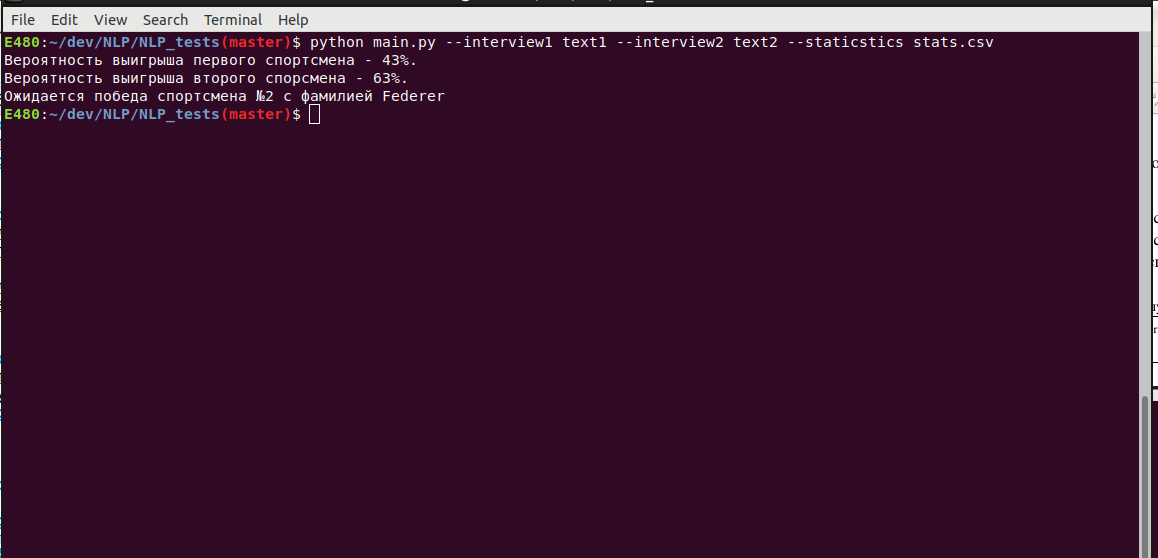
\includegraphics[scale=0.5]{master_img/sample_program.png}
	\caption{Пример работы программы}
	\label{fig10}
\end{figure}
\chapter{Экспериментальный раздел}
\label{cha:research}

В данном разделе проводятся вычислительные эксперименты.
%А на рис.~\ref{fig:spire01} показана схема мыслительного процесса автора...

%\begin{figure}
 % \centering
%  \includegraphics[width=\textwidth]{inc/svg/pic01}
 % \caption{Как страшно жить}
%  \label{fig:spire01}
%\end{figure}


%%% Local Variables:
%%% mode: latex
%%% TeX-master: "rpz"
%%% End:

\chapter{Организационно-экономический раздел}
\label{cha:econom}

\section{Протестируем специальные символы.}

И заодно переключение шрифтов.


{\shorthandoff" \texttt{"-{}-* Прямая речь "-{}-{}- <{}<после ,{},тире`{}` неразрывный пробел>{}>}}

{\cyrillicfonttt{\bfseries\itshape\textbackslash{}cyrillicfonttt}
"--* Прямая речь "--- <<после ,,тире`` неразрывный пробел>>.}

{\cyrillicfontsf{\bfseries\itshape\textbackslash{}cyrillicfontsf}
"--* Прямая речь "--- <<после ,,тире`` неразрывный пробел>>.}

{\cyrillicfont{\bfseries\itshape\textbackslash{}cyrillicfont}
"--* Прямая речь "--- <<после ,,тире`` неразрывный пробел>>.}


\blindtext
%%% Local Variables:
%%% mode: latex
%%% TeX-master: "rpz"
%%% End:

\chapter{Промышленная экология и безопасность}\label{cha:bzd}

\blindtext

\blindlistlist[3]{enumerate}

%%% Local Variables:
%%% mode: latex
%%% TeX-master: "rpz"
%%% End:


\backmatter %% Здесь заканчивается нумерованная часть документа и начинаются ссылки и
            %% заключение

\Conclusion % заключение к отчёту

\begin{figure}
В данной работе были реализованы различные алгоритмы дизеринга, было произведено сравнение и анализ этих алгоритмов. Программа позволяет получить изображение схожего визуального качества при значительном уменьшении размера. Был получен вывод о том, что для различных целей следует использовать различные алгоритмы дизеринга, универсального алгоритма дизеринга не существует. Программа не привязана к какой-то конкретной
операционной системе и может быть скомпилирована и запущена на
всех популярных ОС.
\end{figure}
%%% Local Variables: 
%%% mode: latex
%%% TeX-master: "rpz"
%%% End: 


% % Список литературы при помощи BibTeX
% Юзать так:
%
% pdflatex rpz
% bibtex rpz
% pdflatex rpz

\bibliographystyle{gost780u}
\bibliography{rpz}


%%% Local Variables: 
%%% mode: latex
%%% TeX-master: "rpz"
%%% End: 


\appendix   % Тут идут приложения

%\chapter{Рисунки, поясняющие работу некоторых функций}
%\label{cha:appendix1}

%\begin{figure}
%\centering
%\caption{Картинка в приложении. Страшная и ужасная.}
%\end{figure}

%%% Local Variables: 
%%% mode: latex
%%% TeX-master: "rpz"
%%% End: 

%\chapter{Еще картинки}
%\label{cha:appendix2}

%\begin{figure}
%\centering
%\caption{Еще одна картинка, ничем не лучше предыдущей. Но %надо же как-то заполнить место.}
%\end{figure}

%%% Local Variables: 
%%% mode: latex
%%% TeX-master: "rpz"
%%% End: 


\end{document}

%%% Local Variables:
%%% mode: latex
%%% TeX-master: t
%%% End:
